\section{Examples}

\subsection{Advanced Lists and Enumerations}

Lists are fundamental for structuring information in academic writing. LaTeX provides powerful list environments with extensive customization options.

\subsubsection{Nested Lists}

Lists can be nested up to four levels deep, mixing different types:

\begin{enumerate}
    \item First level enumeration
          \begin{itemize}
              \item Second level bullet point
              \item Another bullet point
                    \begin{enumerate}
                        \item Third level numbered item
                        \item Another numbered item
                              \begin{itemize}
                                  \item Fourth level bullet
                                  \item Maximum nesting depth
                              \end{itemize}
                    \end{enumerate}
              \item Back to second level
          \end{itemize}
    \item Second main point
          \begin{enumerate}[label=\alph*)]
              \item Alphabetic labeling
              \item Useful for sub-points
                    \begin{enumerate}[label=\roman*.]
                        \item Roman numerals
                        \item Classic academic style
                    \end{enumerate}
          \end{enumerate}
\end{enumerate}

\subsubsection{Description Lists}

Description lists are ideal for definitions and glossaries:

\begin{description}
    \item[Machine Learning] A subset of artificial intelligence that enables systems to learn and improve from experience without being explicitly programmed.

    \item[Deep Learning] A machine learning technique based on artificial neural networks with multiple layers between input and output.

    \item[Neural Network] A computing system inspired by biological neural networks, consisting of interconnected nodes (neurons) that process information.

    \item[Gradient Descent] An optimization algorithm used to minimize the cost function by iteratively moving in the direction of steepest descent.
\end{description}

\subsubsection{Custom Enumeration Styles}

The enumitem package allows extensive customization:

\begin{enumerate}[label=\textbf{Step \arabic*:}, leftmargin=*]
    \item \textbf{Data Collection} -- Gather relevant datasets from reliable sources
    \item \textbf{Preprocessing} -- Clean and normalize the data
    \item \textbf{Feature Engineering} -- Extract meaningful features
    \item \textbf{Model Training} -- Train the machine learning model
    \item \textbf{Evaluation} -- Assess model performance using metrics
    \item \textbf{Deployment} -- Integrate the model into production
\end{enumerate}

\subsubsection{Inline Lists}

For lists within paragraphs, use inline enumeration: The process consists of \begin{enumerate*}[label=(\alph*)] \item data acquisition, \item preprocessing, \item analysis, and \item visualization\end{enumerate*}. This format saves space while maintaining clarity.

\subsubsection{Resume and Continue Lists}

Lists can be interrupted and resumed:

\begin{enumerate}
    \item First item in the initial list
    \item Second item before interruption
\end{enumerate}

Some intervening text or other content can appear here, such as explanations, figures, or tables.

\begin{enumerate}[resume]
    \item Third item, continuing the numbering
    \item Fourth item maintaining sequence
\end{enumerate}

\subsubsection{Compact Lists}

For space-efficient lists, reduce spacing:

\begin{itemize}[noitemsep,topsep=0pt]
    \item Compact item with minimal spacing
    \item Another item with reduced gap
    \item Third item in compressed format
    \item Final item maintaining density
\end{itemize}

\subsubsection{Check Lists}

Task lists for thesis milestones:

\begin{itemize}
    \item[$\square$] Literature review completed
    \item[$\square$] Research methodology defined
    \item[$\boxtimes$] Data collection finished
    \item[$\boxtimes$] Initial analysis performed
    \item[$\square$] Results validated
    \item[$\square$] Thesis draft written
\end{itemize}

List formatting best practices:
\begin{itemize}
    \item Maintain consistent punctuation across items
    \item Use parallel grammatical structure
    \item Keep items at similar levels of detail
    \item Choose appropriate list type for content
    \item Limit nesting to maintain readability
    \item Consider using description lists for terminology
\end{itemize}

\subsection{Cross-References with Cleveref}

The cleveref package provides intelligent cross-referencing that automatically includes the reference type (e.g., "Section", "Table", "Figure"). Always use \verb+\cref{}+ instead of \verb+\ref{}+ for better formatting.

Key commands:
\begin{itemize}
    \item \verb+\cref{label}+ for single references with type (e.g., "Section 2.1")
    \item \verb+\Cref{label}+ for capitalized references at sentence beginning
    \item \verb+\cref{label1,label2,label3}+ for multiple references
    \item \verb+\cpageref{label}+ for page references
\end{itemize}

Examples of cross-references using labels from this document:

As shown in \cref{tab:performance}, Algorithm B performs best with 94.7\% accuracy. \Cref{tab:resources} demonstrates system behavior under different loads. Both \cref{tab:performance,tab:resources} use the booktabs package for professional formatting.

\subsection{Including Images}

LaTeX provides excellent support for including external images through the graphicx package. Images should be placed in the \verb+content/images/+ directory for better organization.

Key commands:
\begin{itemize}
    \item \verb+\includegraphics{filename}+ includes an image
    \item \verb+\includegraphics[options]{filename}+ includes an image with formatting options
    \item Common options: \verb+width+, \verb+height+, \verb+scale+, \verb+angle+
    \item Always wrap images in \verb+figure+ environment for proper positioning and captions
\end{itemize}

\subsubsection{Basic Image Inclusion}

Here's an example of including an image with proper sizing and captioning:

\begin{figure}[htbp]
    \centering
    \includegraphics[width=0.6\textwidth]{content/images/logo.jpg}
    \caption{Example logo demonstrating image inclusion in LaTeX documents. The image is scaled to 60\% of the text width for optimal presentation.}
    \label{fig:example_logo}
\end{figure}

As demonstrated in \cref{fig:example_logo}, images are automatically centered and properly integrated into the document flow.

Common sizing options:
\begin{itemize}
    \item \verb+width=0.5\textwidth+ scales to 50\% of text width
    \item \verb+height=5cm+ sets absolute height
    \item \verb+scale=0.8+ scales to 80\% of original size
    \item \verb+width=\linewidth+ fills the entire line width
\end{itemize}

Additional formatting options:
\begin{itemize}
    \item \verb+angle=90+ rotates the image by 90 degrees
    \item \verb+trim=left bottom right top, clip+ crops the image
    \item \verb+keepaspectratio+ maintains aspect ratio when specifying both width and height
\end{itemize}

Best practices for images:
\begin{itemize}
    \item Use vector formats (PDF, SVG) when possible for scalability
    \item For photographs, use high-resolution JPEG or PNG files
    \item Always provide descriptive captions that explain the image content
    \item Use consistent sizing throughout your document
    \item Place images logically within the text flow and reference them appropriately
\end{itemize}

\subsection{Tables with Booktabs}

The booktabs package provides professional-looking tables with proper horizontal lines. Use \verb+\toprule+, \verb+\midrule+, and \verb+\bottomrule+ instead of \verb+\hline+.

Key commands:
\begin{itemize}
    \item \verb+\toprule+ for the top line of the table
    \item \verb+\midrule+ for separating header from content
    \item \verb+\bottomrule+ for the bottom line of the table
    \item \verb+\cmidrule{i-j}+ for partial rules spanning columns i through j
\end{itemize}

Example of a simple table:

\begin{table}[htbp]
    \centering
    \caption{Performance comparison of different algorithms}
    \label{tab:performance}
    \begin{tabular}{lcc}
        \toprule
        Algorithm   & Runtime (ms) & Accuracy (\%) \\
        \midrule
        Algorithm A & 125          & 92.3          \\
        Algorithm B & 98           & 94.7          \\
        Algorithm C & 156          & 89.1          \\
        \bottomrule
    \end{tabular}
\end{table}

Example with grouped columns and partial rules:

\begin{table}[htbp]
    \centering
    \caption{System resource utilization under different workloads}
    \label{tab:resources}
    \begin{tabular}{lcccc}
        \toprule
                    & \multicolumn{2}{c}{Low Load} & \multicolumn{2}{c}{High Load}                       \\
        \cmidrule(lr){2-3} \cmidrule(lr){4-5}
        Component   & CPU (\%)                     & RAM (\%)                      & CPU (\%) & RAM (\%) \\
        \midrule
        Web Server  & 15.2                         & 32.1                          & 78.4     & 65.3     \\
        Database    & 8.7                          & 45.6                          & 45.2     & 82.9     \\
        Cache Layer & 3.1                          & 12.4                          & 23.8     & 34.7     \\
        \bottomrule
    \end{tabular}
\end{table}

\subsection{Bibliography Citations}

Use the \verb+\cite{}+ command to reference entries from your \verb+literature.bib+ file. The ACM citation style provides numbered citations with full author names.

Citation commands for biblatex:
\begin{itemize}
    \item \verb+\cite{key}+ for basic citations [1]
    \item \verb+\textcite{key}+ for textual citations: "Author [1] states..."
    \item \verb+\parencite{key}+ for parenthetical citations (Author [1])
    \item \verb+\footcite{key}+ for footnote citations
\end{itemize}

Examples using references from literature.bib:

The foundational work by~\cite{sample_reference_2020} established the theoretical framework. Recent studies~\cite{another_reference_2021,recent_study_1} have extended this research. For implementation details, see the technical report~\footcite{example_study_1}.

\textcite{foundational_reference_1} documented different approaches in conference proceedings, while \textcite{example_study_2} provided insights in recent dissertations. Current trends are analyzed in \parencite{trend_reference}, and methodological considerations are discussed in \cite{qualitative_example,mixed_methods_example}.

Research gaps have been identified in multiple studies~\cite{gap_evidence_1,gap_evidence_2,gap_evidence_3}, indicating areas for future investigation.

Multiple citations can be grouped:~\cite{sample_reference_2020,another_reference_2021,recent_study_1}.

Note: The ACM style uses numbered citations with full bibliographic details. Ensure you run the complete build process (pdflatex → biber → pdflatex → pdflatex) for proper citation formatting.

\subsection{Footnotes and Annotations}

Footnotes provide supplementary information without disrupting the main text flow, essential for academic writing.

\subsubsection{Basic Footnotes}

Footnotes are created with the \verb+\footnote{}+ command. They appear at the bottom of the page with automatic numbering\footnote{This is a basic footnote example. Footnotes are numbered automatically and reset each chapter.}. You can place footnotes anywhere in the text\footnote{Including multiple footnotes on the same page. LaTeX handles the spacing and positioning automatically.}.

Complex footnotes can contain multiple sentences and even citations\footnote{For detailed analysis of this topic, see recent research~\cite{sample_reference_2020}. This approach has been validated in multiple studies and is now considered standard practice in the field. Note that footnotes can span multiple lines without issues.}.

\subsubsection{Footnotes in Special Contexts}

When using footnotes in tables, place them after the table environment:

\begin{table}[htbp]
    \centering
    \caption{Performance metrics with various optimization levels}
    \label{tab:footnote_example}
    \begin{tabular}{lcc}
        \toprule
        Method        & Accuracy & Speed$^a$ \\
        \midrule
        Baseline      & 85.2\%   & 100 ms    \\
        Optimized$^b$ & 87.9\%   & 75 ms     \\
        Advanced      & 91.3\%   & 150 ms    \\
        \bottomrule
    \end{tabular}

    \vspace{0.5em}
    \footnotesize
    $^a$ Speed measured as average inference time per sample\\
    $^b$ Optimized using automated hyperparameter tuning
\end{table}

\subsubsection{Mathematical Footnotes}

Footnotes can contain mathematical expressions\footnote{The formula $E = mc^2$ demonstrates mass-energy equivalence, where $c \approx 3 \times 10^8$ m/s.} and complex equations\footnote{The solution to the quadratic equation $ax^2 + bx + c = 0$ is given by:
    $$x = \frac{-b \pm \sqrt{b^2 - 4ac}}{2a}$$
    This formula is valid when $a \neq 0$.}.

\subsubsection{URL and Reference Footnotes}

Long URLs are often placed in footnotes to maintain text readability\footnote{\url{https://www.example.com/very/long/path/to/specific/resource/that/would/disrupt/reading/flow}}. Similarly, extended references or clarifications work well in footnotes\footnote{This concept was first introduced by Smith (1970), later refined by Johnson (1985), and finally formalized in the comprehensive framework presented by Williams et al. (2010). For a complete historical overview, see Anderson (2020).}.

\subsubsection{Margin Notes}

While less common in theses, margin notes can be useful for draft annotations. The \verb+\marginpar{}+ command creates notes in the margin:\marginpar{This appears in the margin} though their use should be limited in final documents.

Best practices for footnotes:
\begin{itemize}
    \item Keep footnotes concise and relevant
    \item Avoid excessive footnotes that distract from main text
    \item Use consistent formatting within footnotes
    \item Number footnotes per chapter or continuously as required
    \item Consider whether information belongs in footnote or main text
    \item Ensure footnotes are complete sentences with proper punctuation
\end{itemize}

\subsection{Mathematical Equations}

LaTeX provides exceptional support for mathematical typesetting through the amsmath package. Equations can be displayed inline or in display mode, numbered or unnumbered.

\subsubsection{Inline Mathematics}

For mathematical expressions within text, use \verb+$...$+ or \verb+\(...\)+: The quadratic formula has solutions $x = \frac{-b \pm \sqrt{b^2 - 4ac}}{2a}$ when the discriminant $\Delta = b^2 - 4ac \geq 0$. Euler's identity states that $e^{i\pi} + 1 = 0$.

\subsubsection{Display Equations}

For important equations that deserve their own line, use the equation environment:

\begin{equation}
    E = mc^2
    \label{eq:einstein}
\end{equation}

The mass-energy equivalence shown in \cref{eq:einstein} revolutionized physics. For multiple aligned equations, use the align environment:

\begin{align}
    \nabla \cdot \mathbf{E}  & = \frac{\rho}{\epsilon_0} \label{eq:gauss}                                                  \\
    \nabla \cdot \mathbf{B}  & = 0 \label{eq:gauss_mag}                                                                    \\
    \nabla \times \mathbf{E} & = -\frac{\partial \mathbf{B}}{\partial t} \label{eq:faraday}                                \\
    \nabla \times \mathbf{B} & = \mu_0\mathbf{J} + \mu_0\epsilon_0\frac{\partial \mathbf{E}}{\partial t} \label{eq:ampere}
\end{align}

Maxwell's equations (\cref{eq:gauss,eq:gauss_mag,eq:faraday,eq:ampere}) describe electromagnetic phenomena.

\subsubsection{Mathematical Notation Examples}

Common mathematical constructs for thesis writing:

Summations and products:
\begin{equation}
    \sum_{i=1}^{n} i = \frac{n(n+1)}{2}, \quad \prod_{k=1}^{n} k = n!
\end{equation}

Limits and integrals:
\begin{equation}
    \lim_{x \to \infty} \left(1 + \frac{1}{x}\right)^x = e, \quad \int_{-\infty}^{\infty} e^{-x^2} dx = \sqrt{\pi}
\end{equation}

Matrices and vectors:
\begin{equation}
    \mathbf{A} = \begin{bmatrix}
        a_{11} & a_{12} & \cdots & a_{1n} \\
        a_{21} & a_{22} & \cdots & a_{2n} \\
        \vdots & \vdots & \ddots & \vdots \\
        a_{m1} & a_{m2} & \cdots & a_{mn}
    \end{bmatrix}, \quad
    \mathbf{x} = \begin{pmatrix}
        x_1    \\
        x_2    \\
        \vdots \\
        x_n
    \end{pmatrix}
\end{equation}

Statistical notation:
\begin{equation}
    \bar{x} = \frac{1}{n}\sum_{i=1}^{n} x_i, \quad \sigma^2 = \frac{1}{n-1}\sum_{i=1}^{n} (x_i - \bar{x})^2
\end{equation}

\subsection{Subfigures for Comparisons}

The subcaption package enables side-by-side figure comparisons, essential for presenting related images, before/after comparisons, or multiple experimental results.

\subsubsection{Basic Subfigures}

Use the subfigure environment within a figure to create labeled subfigures:

\begin{figure}[htbp]
    \centering
    \begin{subfigure}[b]{0.45\textwidth}
        \centering
        \includegraphics[width=\textwidth]{content/images/logo.jpg}
        \caption{Original image showing the logo at full resolution}
        \label{fig:logo_original}
    \end{subfigure}
    \hfill
    \begin{subfigure}[b]{0.45\textwidth}
        \centering
        \includegraphics[width=\textwidth,angle=180]{content/images/logo.jpg}
        \caption{Rotated version demonstrating image transformation}
        \label{fig:logo_rotated}
    \end{subfigure}
    \caption{Comparison of image transformations using subfigures. \Cref{fig:logo_original} shows the original, while \cref{fig:logo_rotated} demonstrates a 180-degree rotation.}
    \label{fig:logo_comparison}
\end{figure}

\subsubsection{Multiple Subfigures in Grid Layout}

For comparing multiple results, arrange subfigures in a grid:

\begin{figure}[htbp]
    \centering
    \begin{subfigure}[b]{0.3\textwidth}
        \centering
        \includegraphics[width=\textwidth]{content/images/logo.jpg}
        \caption{Baseline}
        \label{fig:grid_baseline}
    \end{subfigure}
    \hfill
    \begin{subfigure}[b]{0.3\textwidth}
        \centering
        \includegraphics[width=\textwidth,angle=90]{content/images/logo.jpg}
        \caption{90° rotation}
        \label{fig:grid_90}
    \end{subfigure}
    \hfill
    \begin{subfigure}[b]{0.3\textwidth}
        \centering
        \includegraphics[width=\textwidth,angle=270]{content/images/logo.jpg}
        \caption{270° rotation}
        \label{fig:grid_270}
    \end{subfigure}

    \begin{subfigure}[b]{0.3\textwidth}
        \centering
        \includegraphics[width=\textwidth,scale=0.5]{content/images/logo.jpg}
        \caption{50\% scale}
        \label{fig:grid_scale50}
    \end{subfigure}
    \hfill
    \begin{subfigure}[b]{0.3\textwidth}
        \centering
        \includegraphics[width=\textwidth,scale=0.75]{content/images/logo.jpg}
        \caption{75\% scale}
        \label{fig:grid_scale75}
    \end{subfigure}
    \hfill
    \begin{subfigure}[b]{0.3\textwidth}
        \centering
        \includegraphics[width=\textwidth,scale=1.25]{content/images/logo.jpg}
        \caption{125\% scale}
        \label{fig:grid_scale125}
    \end{subfigure}
    \caption{Grid layout demonstrating multiple image transformations for systematic comparison of experimental results.}
    \label{fig:grid_comparison}
\end{figure}

Key subfigure commands:
\begin{itemize}
    \item \verb+\begin{subfigure}[position]{width}+ creates a subfigure environment
    \item \verb+[b]+ aligns subfigures at bottom, \verb+[t]+ at top, \verb+[c]+ at center
    \item \verb+\hfill+ creates horizontal space between subfigures
    \item Each subfigure can have its own \verb+\caption{}+ and \verb+\label{}+
    \item Reference individual subfigures with \verb+\cref{label}+
\end{itemize}

Best practices for subfigures:
\begin{itemize}
    \item Keep subfigure widths consistent for visual balance
    \item Use \verb+\hfill+ or \verb+\hspace{}+ for proper spacing
    \item Provide descriptive subcaptions that explain differences
    \item Reference both the main figure and specific subfigures in text
    \item Consider using \verb+[htbp]+ placement for better float positioning
\end{itemize}

\subsection{Data Visualization with PGFPlots}

The pgfplots package provides powerful tools for creating high-quality plots and charts directly in LaTeX. It builds on TikZ and offers excellent integration with the document's typography and styling.

Key features:
\begin{itemize}
    \item \verb+axis+ environment for creating coordinate systems
    \item \verb+\addplot+ for adding data series
    \item Automatic legend generation with \verb+\addlegendentry+
    \item Support for various plot types: line plots, scatter plots, bar charts, etc.
    \item Data input from coordinates, tables, or mathematical functions
\end{itemize}

\subsubsection{Creating Line Plots}

PGFPlots excels at creating scientific plots with precise control over appearance. The following example demonstrates a performance comparison chart:

\begin{figure}[htbp]
    \centering
    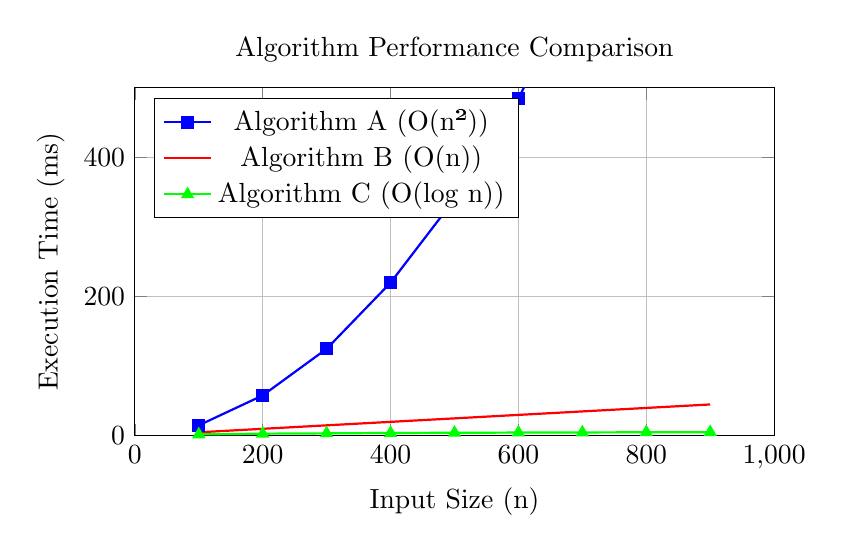
\begin{tikzpicture}
        \begin{axis}[
                title={Algorithm Performance Comparison},
                xlabel={Input Size (n)},
                ylabel={Execution Time (ms)},
                width=0.8\textwidth,
                height=6cm,
                grid=major,
                legend pos=north west,
                xmin=0, xmax=1000,
                ymin=0, ymax=500
            ]

            % Algorithm A - Quadratic complexity
            \addplot[color=blue, mark=square*, thick] coordinates {
                    (100, 15)
                    (200, 58)
                    (300, 125)
                    (400, 220)
                    (500, 340)
                    (600, 485)
                    (700, 665)
                    (800, 875)
                    (900, 1115)
                };
            \addlegendentry{Algorithm A (O(n²))}

            % Algorithm B - Linear complexity
            \addplot[color=red, mark=circle*, thick] coordinates {
                    (100, 5)
                    (200, 10)
                    (300, 15)
                    (400, 20)
                    (500, 25)
                    (600, 30)
                    (700, 35)
                    (800, 40)
                    (900, 45)
                };
            \addlegendentry{Algorithm B (O(n))}

            % Algorithm C - Logarithmic complexity
            \addplot[color=green, mark=triangle*, thick] coordinates {
                    (100, 2)
                    (200, 3)
                    (300, 3.5)
                    (400, 4)
                    (500, 4.3)
                    (600, 4.6)
                    (700, 4.8)
                    (800, 5)
                    (900, 5.2)
                };
            \addlegendentry{Algorithm C (O(log n))}

        \end{axis}
    \end{tikzpicture}
    \caption{Performance comparison showing different algorithmic complexities. Algorithm C demonstrates the best scalability with logarithmic growth, while Algorithm A shows quadratic growth limiting its use for large datasets.}
    \label{fig:performance_comparison}
\end{figure}


As shown in \cref{fig:performance_comparison}, different algorithms exhibit distinct growth patterns. The logarithmic complexity of Algorithm C makes it suitable for large-scale applications, while the quadratic growth of Algorithm A limits scalability.

Common pgfplots options:
\begin{itemize}
    \item \verb+title+ sets the plot title
    \item \verb+xlabel+ and \verb+ylabel+ label the axes
    \item \verb+grid=major+ adds a grid for better readability
    \item \verb+legend pos+ controls legend positioning
    \item \verb+width+ and \verb+height+ control plot dimensions
    \item \verb+xmin+, \verb+xmax+, \verb+ymin+, \verb+ymax+ set axis ranges
\end{itemize}

Plot styling options include:
\begin{itemize}
    \item \verb+color+ for line colors
    \item \verb+mark+ for data point markers (circle*, square*, triangle*, etc.)
    \item \verb+thick+ or \verb+ultra thick+ for line width
    \item \verb+dashed+ or \verb+dotted+ for line patterns
\end{itemize}

PGFPlots automatically handles axis scaling, tick marks, and provides professional-quality output that matches your document's fonts and styling.

\subsection{Code Listings with Minted}

The minted package provides syntax highlighting for code listings using the Pygments library. It offers superior highlighting compared to the default listings package.

Key features:
\begin{itemize}
    \item \verb+\mint{language}{code}+ for inline code snippets
    \item \verb+minted+ environment for code blocks
    \item \verb+\inputminted{language}{filename}+ for external files
\end{itemize}

\subsubsection{Direct Code Specification}

Use the minted environment to include code directly in your LaTeX document:

\begin{minted}[linenos,bgcolor=lightgray,frame=lines,framesep=2mm]{python}
def fibonacci(n):
    """Calculate the nth Fibonacci number."""
    if n <= 1:
        return n
    return fibonacci(n-1) + fibonacci(n-2)

# Example usage
result = fibonacci(10)
print(f"The 10th Fibonacci number is: {result}")
\end{minted}

\subsubsection{Inline Code}

For short code snippets within text, use \verb+\mint{}{}+ or \verb+\mintinline{}{}+:

The function \mintinline{python}{len(list)} returns the length of a list.
For JSON parsing, use \mintinline{javascript}{JSON.parse(data)}.
Database queries can be written as \verb|SELECT * FROM users WHERE active = 1|.

\subsubsection{External File Input}

For larger code files, use \verb+\inputminted{}{}+ to include external source files:

\inputminted[linenos,bgcolor=lightgray,frame=lines,framesep=2mm]{javascript}{content/scripts/example.js}

Common minted options:
\begin{itemize}
    \item \verb+linenos+ adds line numbers
    \item \verb+bgcolor+ sets background color
    \item \verb+frame+ adds a frame around the code
    \item \verb+framesep+ controls frame separation
    \item \verb+fontsize+ adjusts the font size
    \item \verb+breaklines+ enables automatic line breaking
\end{itemize}

Note: Minted requires the \verb+-shell-escape+ flag when compiling with pdflatex.

\subsection{Algorithm Pseudocode}

The algorithm and algpseudocode packages provide professional formatting for algorithms, essential for computer science and engineering theses.

\subsubsection{Basic Algorithm}

Here's an example of a sorting algorithm:

\begin{algorithm}[htbp]
    \caption{QuickSort Algorithm}
    \label{alg:quicksort}
    \begin{algorithmic}[1]
        \Require Array $A$ of comparable elements, indices $low$, $high$
        \Ensure Array $A$ is sorted in ascending order between indices $low$ and $high$
        \Procedure{QuickSort}{$A, low, high$}
        \If{$low < high$}
        \State $pivot \gets$ \Call{Partition}{$A, low, high$}
        \State \Call{QuickSort}{$A, low, pivot - 1$}
        \State \Call{QuickSort}{$A, pivot + 1, high$}
        \EndIf
        \EndProcedure
        \Procedure{Partition}{$A, low, high$}
        \State $pivot \gets A[high]$
        \State $i \gets low - 1$
        \For{$j \gets low$ \textbf{to} $high - 1$}
        \If{$A[j] \leq pivot$}
        \State $i \gets i + 1$
        \State \textbf{swap} $A[i]$ and $A[j]$
        \EndIf
        \EndFor
        \State \textbf{swap} $A[i + 1]$ and $A[high]$
        \State \Return $i + 1$
        \EndProcedure
    \end{algorithmic}
\end{algorithm}

\subsubsection{Machine Learning Algorithm}

A more complex example showing a gradient descent algorithm:

\begin{algorithm}[htbp]
    \caption{Stochastic Gradient Descent for Neural Network Training}
    \label{alg:sgd}
    \begin{algorithmic}[1]
        \Require Training data $\{(x_i, y_i)\}_{i=1}^n$, learning rate $\alpha$, epochs $E$, batch size $B$
        \Ensure Trained model parameters $\theta$
        \State Initialize parameters $\theta$ randomly
        \State Initialize epoch counter $e \gets 0$
        \While{$e < E$ \textbf{and not} converged}
        \State Shuffle training data
        \For{each mini-batch $\mathcal{B}$ of size $B$}
        \State $g \gets \vec{0}$ \Comment{Initialize gradient}
        \For{each $(x, y) \in \mathcal{B}$}
        \State $\hat{y} \gets$ \Call{Forward}{$x, \theta$} \Comment{Forward pass}
        \State $\ell \gets$ \Call{ComputeLoss}{$\hat{y}, y$}
        \State $g \gets g + \nabla_\theta \ell$ \Comment{Accumulate gradients}
        \EndFor
        \State $g \gets g / |\mathcal{B}|$ \Comment{Average gradients}
        \State $\theta \gets \theta - \alpha \cdot g$ \Comment{Update parameters}
        \If{validation loss increases}
        \State $\alpha \gets \alpha \cdot 0.9$ \Comment{Learning rate decay}
        \EndIf
        \EndFor
        \State $e \gets e + 1$
        \EndWhile
        \State \Return $\theta$
    \end{algorithmic}
\end{algorithm}

\subsubsection{Graph Algorithm}

Demonstrating breadth-first search with proper formatting:

\begin{algorithm}[htbp]
    \caption{Breadth-First Search (BFS)}
    \label{alg:bfs}
    \begin{algorithmic}[1]
        \Require Graph $G = (V, E)$, source vertex $s$
        \Ensure Distance array $d$ and parent array $\pi$
        \ForAll{$v \in V \setminus \{s\}$}
        \State $d[v] \gets \infty$
        \State $\pi[v] \gets$ \textsc{nil}
        \EndFor
        \State $d[s] \gets 0$
        \State $\pi[s] \gets$ \textsc{nil}
        \State $Q \gets \emptyset$ \Comment{Initialize empty queue}
        \State \Call{Enqueue}{$Q, s$}
        \While{$Q \neq \emptyset$}
        \State $u \gets$ \Call{Dequeue}{$Q$}
        \ForAll{$v \in \text{Adj}[u]$}
        \If{$d[v] = \infty$}
        \State $d[v] \gets d[u] + 1$
        \State $\pi[v] \gets u$
        \State \Call{Enqueue}{$Q, v$}
        \EndIf
        \EndFor
        \EndWhile
    \end{algorithmic}
\end{algorithm}

Key algorithm commands:
\begin{itemize}
    \item \verb+\begin{algorithm}+ creates a floating algorithm environment
    \item \verb+\begin{algorithmic}[1]+ starts pseudocode with line numbering
    \item \verb+\State+ for single statements
    \item \verb+\If{condition}...\EndIf+ for conditionals
    \item \verb+\For{condition}...\EndFor+ for loops
    \item \verb+\While{condition}...\EndWhile+ for while loops
    \item \verb+\Procedure{name}{params}...\EndProcedure+ for procedures
    \item \verb+\Call{function}{params}+ for function calls
    \item \verb+\Comment{text}+ for inline comments
\end{itemize}

As shown in \cref{alg:quicksort}, algorithms can be referenced like figures and tables. The SGD algorithm (\cref{alg:sgd}) demonstrates more complex control flow, while \cref{alg:bfs} shows graph traversal notation.

\subsection{Acronyms}

The acronym package controls first and subsequent mentions automatically:

\begin{itemize}
    \item \verb+\ac{LABEL}+ prints "Long form (ABBR)" on first use, then "ABBR".
    \item \verb+\acs{LABEL}+ prints only the abbreviation.
    \item \verb+\acl{LABEL}+ prints only the long form.
    \item \verb+\acp{LABEL}+ pluralizes when supported.
\end{itemize}

Examples:

\ac{AES} protects data at rest. Many workloads run on a \ac{CPU} or a \ac{GPU}. Data is stored in \ac{RAM}. Services expose an \ac{API} over \ac{HTTP}. For transport, \ac{TCP} and \ac{UDP} are common. Payloads often use \ac{JSON}. Data queries are written in \ac{SQL}.